\fancyhead[LO]{{\scriptsize {\FA \ }我们最幸福 {\FA } 在黑暗中手牵着手}}%奇數頁眉的左邊
\fancyhead[RO]{{\tiny{\textcolor{Gray}{\FA \ }}}\thepage}
\fancyhead[LE]{{\tiny{\textcolor{Gray}{\FA \ }}}\thepage}
\fancyhead[RE]{{\scriptsize {\FA }我们最幸福 {\FA } 在黑暗中手牵着手}}%偶數頁眉的右邊
\fancyfoot[LE,RO]{}
\fancyfoot[LO,CE]{}
\fancyfoot[CO,RE]{}
\chapter*{01 {\FA } 在黑暗中手牵着手}
\addcontentsline{toc}{chapter}{\hspace{5mm}01 \textbf{>}\ \ 在黑暗中手牵着手}
\begin{flushright}
	\textcolor{PinYinColor}{\EN \huge{Holding Hands\\
		in the Dark\\
	\ \\}}
\end{flushright}
\begin{figure}[!htbp]
	\centering
	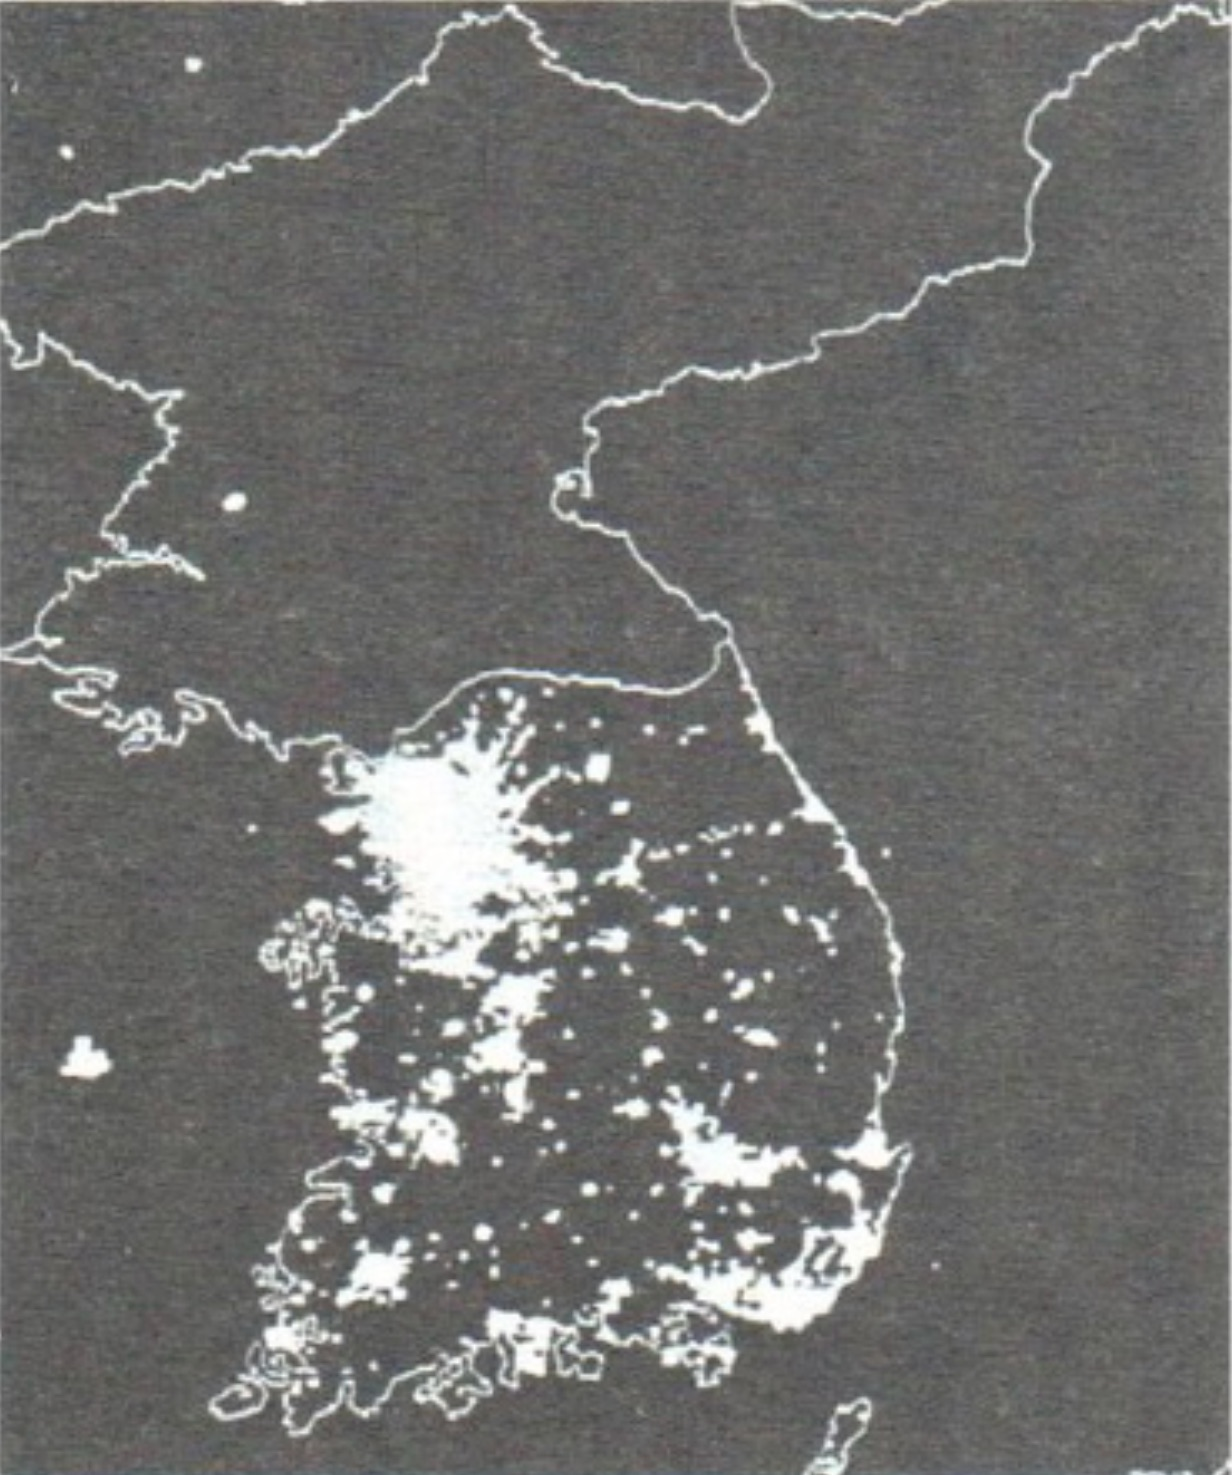
\includegraphics[width=6cm]{./Chapters/Images/01.jpg}
	\caption*{北朝鲜及南韩的夜间卫星照片}
\end{figure}

如果看一下远东地区夜间的卫星照片,你会发现有一大片的地区很奇怪的没有亮光。这片处于黑暗的地区就是朝鲜人民民主主义人民共和国的所在。\\

与这个神秘黑洞接壤的南韩、日本及现在的中国都闪烁着代表着繁荣的亮光。即使从数百公里以上的高空看下来,广告牌、车灯、街灯及连锁快餐店的霓虹灯都变成一个个细小的光点,显示着人们作为21世纪的能源消费者在各自忙绿着。然而在这其中,却有着一个近乎英格兰大小的黑暗地带。难以置信的是一个拥有大概2300万人口的国家,表现出来的却是和周围海洋一样的真空。然而,北朝鲜就是这样一片空白。\\

北朝鲜大约在90年代初慢慢衰落暗淡的。随着苏联的解体,支撑社会主义联盟的廉价石油不复存在了,北朝鲜脆弱且无效率运转的经济体系也随之崩溃。发电厂设备锈死瘫痪。电灯不再发光。饥饿的人们爬上电线杆,偷取那一点点铜线以换取食物。当夕阳西下,一切都变成了灰色,蹲在地上矮矮的房子也被夜色一点点的吞噬。整个村庄慢慢的消失在暮色之中。即使在首都平壤,这个的橱窗式的城市,夜晚当你漫步于主要街道之时,也无法看清道路两旁的建筑。\\

当外人凝视着今日北朝鲜这一片漆黑的夜晚,他们可能会联想到在遥远的非洲或者东南亚某个文明之手──电,尚未触及的村落。然而北朝鲜却不是一个未开化的国家,它是一个末落的发达国家。沿着任何一条北朝鲜的主干道,抬头即可发现他曾经的辉煌及怎样的失落──那些摇摇欲坠的输电线、锈迹斑斑的铁塔证明着,电网曾经覆盖着整个国家。\\

北朝鲜中年以上年纪的人都记得,曾几何时,他们比在南韩亲美的表亲有着更多的电力\footnote{更多的电力也意味着更多的食物。},然而现在他们却不得不枯坐在黑暗中,心里五味陈杂。回到20世纪90年代,美国曾许诺以能源援助换取北朝鲜放弃核武器计划。然而,这项交易却由于布什政府指责北朝鲜违背承诺而最终告吹。北朝鲜人痛苦的抱怨着缺乏电力所带来的黑暗,进而他们也谴责美国的制裁。晚上,他们不能读书、不能看电视。“没有电,我们根本没有文化生活。”一个粗鲁的北朝鲜警卫曾经没有好气的向我抱怨着。\\

然而,黑暗又有它的好处。尤其是对于那些正与人偷偷约会的青少年来说。\\

当大人们早早上床之后,冬天这个时间可能会早至晚上7点,那就很容易悄悄的溜出来。享受着黑暗所赐予的私密和自由,而这在有电的时期是很难想象的。披着神奇的隐身斗篷,你可以为所欲为而不用担心父母,邻居或者秘密警察那警惕的目光。\\

我遇到很多北朝鲜人,他们告诉我如何努力学会去喜欢黑暗,但是留给我最深印象的还是一个十几岁的女孩和她男友的故事。12岁那一年,她遇到了临镇一个大她3岁的男孩。在北朝鲜拜占庭式的社会管理体系中,她家处于很低的阶层,因而,两人公开在一起的话,不仅会毁掉男孩的前程,也对女孩的清白名声不好。因此,他们只能在黑暗中长久的散步约会。除此之外,也没什么事情可做。他们最初的交往开始于90年代初期,那个时候由于缺乏电力,餐厅或者电影院都关门歇业了。\\

他们会在晚饭后见面。女孩告诉男友不要敲前门,这样会有被她的姐姐、弟弟或者那些爱多管闲事的邻居们发现的危险。他们都挤在一个狭长的建筑里,屋后是户外厕所,由很多家人共享。房子由一座高仅及人视线的围墙同街面隔开。男孩在墙后发现了一块地方,当天色暗下来之后,在这里没有人会注意到他。邻居们洗碗或者冲厕所的哗哗声掩盖了他的脚步声。接下来,他要做的只是等待,这可能是1小时、2小时甚至3小时。这没关系,北朝鲜的生活节奏很慢,也没有人有手表。\\

一旦摆脱家人,女孩会马上出现。步入户外,凝视着前面的黑暗,起初看不到他,但是她能感觉到他就在附近。她不用为化妆而烦恼,黑暗中没有人需要化妆。有时候她就穿着自己的校服,那是一件裁剪适当的宝蓝色裙子,刚刚好掩住膝盖。白衬衣,配着红色的蝴蝶结。所有的衣服都是由一种爱起皱的化纤面料裁剪而成。女孩还没有到为穿着打扮而烦恼的年纪。\\

起初,他们只是默默的走着,接着他们开始窃窃私语,当他们离开了村庄,完全放松在黑暗里之后,耳语就变成普通音量的对话了。直到他们确信没有其它人之前,他们始终保持一臂之距。\\

离开镇子不远,道路通往一片树林,绿树环绕之中有个曾颇有名气的温泉度假村。它55度的泉水曾经吸引着一车又一车寻求治愈关节炎及糖尿病的中国观光客,但是度假村现在却极少营业。在其入口处,有一个用石墙围成的长方形映景池。穿过庭院的大道两旁,种着松树,日本枫树,以及女孩最喜欢的──银杏树,一到秋天,金黄色的落叶随风飘舞,形状宛如东方的折扇。周围山上的树木都被人们作为柴火砍光了,但温泉旁的树木是如此美丽,以至于人们都不忍心砍伐,使得这些树得以保存了下来。\\

然而,庭院的状况保持的不太好。树木无人修剪,石凳也支离破碎,铺路的石块像烂掉的牙齿,参差不齐。在20世纪90年代中期,北朝鲜好像一切都消耗殆尽了、破损了、失灵了。整个国家曾经有过好日子。然而到了夜间,残败的景象就不那么扎眼了。长满杂草的温泉池里,池水清晰的倒映着璀璨的夜空。\\

北朝鲜的夜空是一道难得的景致。它可能是东北亚地区最闪亮的夜空。在亚洲大陆的其它地区充斥着煤灰,戈壁滩的沙尘暴及二氧化碳,而这里可能是唯一的一块净土。在过去,北朝鲜的工厂也为这些白茫茫的烟雾做着贡献,然而现在不会了。现在没有任何人造的光线同夜空中满天的星斗争辉。\\

年轻的情侣在夜色中漫步,脚步带起地上的银杏叶。他们都谈些什么呢?家人、同学、读过的书等等无论什么都可以成为话题,这给他们带来了无尽的欢乐。以至于多年后,当我问这个女孩什么是她一生中最快乐的记忆,她给我讲述了这些夜晚。\\

这一类的事情不可能出现在卫星照片中。无论是在位于弗吉尼亚州拉格雷市的中情局总部,还是在大学的东亚研究部门,人们只是在远远的地方分析北朝鲜。他们可能想不到,在这个黑洞的中间,一个数百万人死于饥荒的黑暗国家里面,原来也有爱情。\\

到我遇到这个女孩的时候,她已经是一个31岁的女人了。美兰(Mi-ran)\footnote{在这本书里,我用美兰这个名字称呼她。}脱离北朝鲜在南韩已经生活了6年。我曾经因为一篇关于脱北者的文章而要求采访她。\\

2004年我被派往首尔,作为《洛杉矶时报》的总编辑。我的工作范围涵盖整个朝鲜半岛。南韩一边的工作很容易开展。作为当时世界第13大经济体,韩国的民主,繁荣还有点喧闹,它有着亚洲最积极的新闻媒体。政府官员也乐意把他们的手机号码给记者们,也不介意下班的时候被打扰。北朝鲜却是另外一个极端。北朝鲜的对外信息传播渠道仅限于北朝鲜中央新闻社所发表那些冗长、措辞激烈的社论。这个机构,因为它关于“美帝国主义”的那些荒谬而夸张的言论,而被戏称为“大辱骂者”。美国在1950-53年爆发的朝鲜战争中为南韩而战,那次战争是冷战中第一次激烈的局部战争,迄今为止美国仍然在南韩留有4万人的驻军。对于北朝鲜而言,战争从未结束,敌意时时刻刻的存在。\\

美国公民鲜有能获准进入北朝鲜的,记者更甚。2005年,当我和一名同事终于拿到北朝鲜签证,得以造访平壤的时候,被带领沿着一条制式的参观线路游览,参观为纪念光辉领袖金正日及他的前任金日成而建的各种纪念碑。在北朝鲜期间,我们一直都由两个身材削瘦的黑衣人陪伴着,他们都叫朴先生\footnote{北朝鲜通常都会采取预防措施,派两名看管,这样他们可以相互监督,以免被收买。}。这些看管们说的话同空虚生硬的官方通讯社保持一致\footnote{例如“感谢我们的领袖金正日”这个短语以令人奇异的频率反复出现在我们的谈话中。}。言谈之间,他们很少同我们进行目光交流,我也怀疑他们是否相信他们所说的内容。他们真正在想什么?他们是不是真的同他们宣传的那样爱戴他们的领袖?他们有没有足够的食物?他们下班后都做什么?在全世界最高压的政权下的生活是怎样的?\\

如果我想得到我这些问题的答案,毫无疑问,从北朝鲜内部是无法获得的。我必须同那些离开的人──脱北者,交谈。\\

2004年美兰住在位于首尔以南30公里的水原(Suwon),那里灯火通明但又杂乱无章。水原是三星电子的总部所在地,聚集着大批制造业工厂。生产着大多数北朝鲜人闻所未闻的产品──计算机监视器、光驱、数码电视和闪存条\footnote{据一项经常被引用的统计数据显示,北朝鲜与南韩之间的经济差距,四倍于1990年两德统一时,东西德之间的差距。}。这个地方很喧闹而拥挤,满是搭配不协调的色彩及刺耳的噪音。与大多数南韩的城市一样,建筑风格都是那种丑陋的混凝土盒子,房顶上挤满眼花缭乱的各种招牌。高层公寓楼从拥挤的城市中心向外延绵数公里。公寓楼之间由甜甜圈(Dunkin{\EN '} Donuts)及必胜客(Pizza Hut),以及更多其它的韩式餐厅相连接。街后面的小巷里,满是名为“爱神旅馆”或“爱之园地”情人旅馆,房间按小时出租。交通状况也是,街道被经济奇迹所创造出的──成千上万的现代汽车挤得水泄不通,人们艰难的在家和大卖场之间慢慢的挪着。鉴于这个城市的交通永远处于永无止境的拥堵之中,我决定搭乘从首尔出发的火车,仅仅30分钟的车程,然后在出租车上蜗行至这个城市为数不多的一处幽静之地,一个烤牛排餐厅,位于一个建于18世纪的古军事城堡的对面。\\

起初,我没有认出美兰。她看上去和我之前见过的北朝鲜人不太一样。当时,在南韩生活着超过6000名来自北朝鲜的脱北者,他们身上往往都带有很明显的破绽,透露着他们在融入当地生活的过程中所遇到的困难──过短的裙子,没有去掉标签的新衣服──但是美兰却同南韩人一无二致。她穿着一件别致的褐色毛衣,配以针织的裤子。这给我端庄的感觉\footnote{我对人的第一印象很多情况都被证明是错误的。}。她的头发整齐的梳到脑后,并用一个镶着水钻的发卡别住。她的面容姣好,只是下巴上略有粉刺,身子也略显沉重,这是怀孕三个月的结果。一年前,美兰同一位供职于南韩军队的文职人员结了婚,现在正期待着他们第一个孩子的降生。\\

我邀请美兰共进午餐,以期了解更多关于北朝鲜学校体系的情况。出逃之前,美兰在一个矿区小镇的幼儿园做过几年教师。现在,美兰在南韩攻读一个教育方面的学位。谈话很沉重,那是一段不堪回首的日子。当谈及那些5-6岁左右的学生们因为饥饿死去的时候,桌子上的饭菜也是一口没碰。当孩子们一个个不断死去的时候,她仍然被要求告诉孩子们,他们是被祝福才生为北朝鲜人的。金日成,从二战结束开始一直到1994年去世为止,北朝鲜的统治者,被尊奉为神。而他的儿子和继任者,金正日,作为神的儿子,是个基督式的人物。美兰对这种北朝鲜系统的洗脑深恶痛绝。\\

谈话进行了一个或两个小时之后,我们的话题就转到一些女孩之间的闲聊了。美兰的沉着和率直也使我问了很多的私人方面的问题。诸如,北朝鲜年轻人的娱乐方式是什么?她在北朝鲜时游过快乐的时光吗?她在那有男友吗?\\

“你问的很有趣。”她说。“我前几天刚好做梦梦见了他。”\\

她告诉我,那个男孩高高瘦瘦的,前额留着浓密的大浏海。离开北朝鲜之后,美兰很高兴的发现在南韩有个青春偶像叫刘俊相的,和她的前男友长得非常像\footnote{基于此点,在这本书里我就用俊相来称呼他。}。他非常聪明,在平壤一所最好的大学里读书,日后有可能成为科学家。这也是他们不能公开恋情的原因之一。他们的关系可能会毁了他的前程。\\

在北朝鲜,没有情人旅馆。异性之间偶尔的亲密行为是很难发生的。但是我还是想委婉的打听一下他们之间的关系到了什么地步。\\

美兰笑了起来。\\

“我们花了3年时间才牵手,又花了另外6年才接吻。”她说道。“我从来不敢想象除此之外还能做什么。我离开北朝鲜的时候都26岁了,但是我却不知道怎么才能怀上孩子的。”\\

美兰承认她经常会想起她的初恋,对于自己不辞而别的离别方式也感到非常痛苦和懊悔。俊相是她最好的朋友,是她可以将梦想、甚至家庭机密相倾述的人。尽管如此,她还是向他保留了人生中最大的一个秘密。她从来没有对他说过她是多么厌恶北朝鲜,同时她也完全不相信那些她教给自己学生的宣传话语。更重要的是,她从来没有告诉他关于她家的逃离计划。这并不是因为她不信任他,而是在北朝鲜,再怎么谨慎都不为过。如果他告诉别人,而别人又告诉其它人,这你从来不会知晓,且在北朝鲜密探无处不在。邻居们相互揭发、朋友揭发朋友甚至恋人都会相互揭发。如果秘密警察对此事有所耳闻,那么她的整个家庭都会被关进囚车,送到大山里的劳动营。\\

“我不能冒那个险。”她告诉我,“我甚至不能去道个别。”\\

在我们的初次会面之后,我和美兰经常谈及俊相。她是一个幸福的已婚女人,在我再次看到她的时候,她已经是一个妈妈了,但是,无论何时当俊相的名字被提及的时候,她的语速就会加快而且还会脸红。我感觉到,美兰很乐意同我谈及此事,因为除我之外,她不能同其它任何人提及到他。\\

“他后来怎么样了?”我问道。\\

她耸了耸肩。朝鲜战争已经结束50年了,南北的朝鲜人却不能相互联系。就此事而言,南北朝鲜同东西德国或者世界上其它类此情况完全不同。北朝鲜和南韩之间不通电话、不通信函甚至电子邮件都无法抵达。\\

美兰自己也有很多不可能得到答案的问题。\\

他结婚了吗?他还想着她吗?他恨她的不辞而别吗?俊相会不会因为她的叛逃而认为她是祖国的叛徒?\\

“我想他会理解我的,但是真的,我却无从知晓。”她答道。\\

美兰和俊相在他们刚刚十几岁的时候就相遇了。他们都住清津市郊,一个位于北朝鲜北部的工业城市,那里离俄罗斯的边境不太远。\\

北朝鲜的景色山川像极了东方的水墨画。以美国人的观点来看,很多地方,美的让人惊叹。同美国西北部太平洋沿岸区域的景色比较类似,只是不知怎么的,缺乏些色彩。色彩仅限于冷杉、杜松、云杉的深绿到花岗岩山峰的浅灰白。亚洲乡村特有的、郁郁葱葱拼图般的稻田,只能在夏季多雨的那几个月才能看见。秋天的时候,树叶迅速失去的颜色。之后,一年里的其它时间都是黄色和棕色,逐渐凋敝。\\

南韩随处可见的凌乱,在这里完全看不到。几乎没有广告牌、没有车辆。在北朝鲜,私人拥有汽车基本上是非法的,也没有人买得起汽车。拖拉机也很少看见,零零散散的都是些黄牛在拉着犁。房子简朴、实用,形制整齐划一。这些房子很少有建于朝鲜战争之前的。主要建筑大多于60-70年代,用水泥、石灰建成,并且根据工作和职务,分配给民众。在城市里,还有很多所谓的“鸽子笼”,就是只有一间房间的低层公寓楼,然而在乡村,人们都住在一种单层的叫“口琴屋”的房子里,那是数排只有一间房间的房子,紧紧贴在一起,就像口琴上的方形气孔。偶尔,门框和窗框会被漆成扎眼的青绿色,但是绝大多数情况,所有的东西都是刷成白色或者灰色的。\\

在反乌托邦\footnote{反理想主义。──译者}小说《1984》里,乔治欧文(George Orwell)描绘了一个世界,在哪里唯一的色彩是出现在宣传画里面。北朝鲜的情况正是如此。金日成的形象用社会主义写实风格以生动的色彩出现在招贴画中。伟大的领袖坐在长凳上,被一群身着艳丽服装的孩子们拥簇着,脸上洋溢着慈祥的微笑。一道道黄色或者橙色的射线从他的脸上射出:他就是太阳。\\

红色是书写那些无处不在的宣传标语的专用色。朝鲜语使用一套独特的,由圈和线组成的字母。在灰色的背景里面,红色的文字就显得特别显眼。他们遍布田野,刻在山崖峭壁中,如里程碑一样不时的出现在主干道旁,晃动在火车站或者其它公共建筑物的屋顶上。\\

\begin{quote}
	金日成万岁!\\
	金正日21世纪的太阳!\\
	走我们自己的路!\\
	党说什么我们做什么!\\
	这个世界上没什么值得我们羡慕的!\\
\end{quote}

少年时代,美兰没有理由不去相信这些宣传。他的父亲是个卑微的矿工,他的家很穷,但是他们所认识的每一个人都是一样的穷。由于外界的出版物、电影、广播又是被严格禁止的。美兰设想世界上应该没有其它地方的人会过的更好。她在广播电视里一次次的听到,在亲美傀儡领导人朴正熙及他的继任者,全斗焕的统治下,南韩人民生活在水深火热之中。他们还得知,中国修正的共产主义远不如金日成所领导的成功,很多中国人都在忍饥挨饿。总而言之,美兰感到很幸运能生在北朝鲜,沐浴在伟大领袖慈父般的关怀之下。\\

事实上在美兰长大的这个小村庄,70-80年代时,条件还是不算差的。这是典型的千把人左右的一个村庄,整个村子像豆腐块一样建设的整整齐齐,由于是集中规划,使得这个小村庄和其它的村庄没什么区别,但是这个村庄却有着的得天独厚的地理位置。10公里外就是东海,所以村民们时不时的还可以吃到新鲜的鱼和蟹。同时,村子坐落于清津市那一排排烟囱的后面,所以村子既靠近城市,又有一些空地可以用来种植蔬菜。这里的地势相对平坦,这在这个国家是非常难得的,金日成众多的度假别墅中,有一栋就坐落于这附近的温泉中。\\

美兰是四姐妹中最小的一个。她出生于1973年,这在北朝鲜简直是个悲剧,有点像19世纪英格兰作家简奥斯汀(Jane Austen)笔下《傲慢与偏见》里,那个不幸有着五个女儿的家庭。南北朝鲜人都尊同儒家文化,认为男孩能够延续家族、传宗接代、抚养老人。在美兰出生之后3年,美兰的父母终于摆脱了没有男孩的窘境,但是这也意味着他们最小的女儿在这个家庭成为一个被遗忘的孩子。\\

根据美兰父亲的情况,一家人住在口琴屋里的一个单间。进门后就是一个小的厨房,也兼炉子间功能。柴火或者煤被铲进炉膛里。炉火既可以用来煮饭,也可以通过一种称为“炕”的地热系统为房间供暖。一扇移门将厨房和主房隔开,一家人都睡在地板上,晚上铺上垫子,白天收起来。随着男孩的降生,家庭成员也扩大到八个人、五个孩子、父母和外婆。因此,美兰的父亲贿赂了人民委员会的头头,将隔壁的一个单元也给了他们,并且同意他们打通了相邻的隔墙。\\

有了更大的空间,家里的男女也就分开了。吃饭时,女人们挤在靠近厨房的一张矮桌旁,吃着玉米饭,玉米饭比北朝鲜人喜爱的主食──白米饭要便宜,但是却不如白米饭有营养。而父亲和儿子却在他们自己的桌子上吃白米饭。\\

“我想生活就应该是这个样子的。”美兰的弟弟,锡柱(Sok-ju)后来告诉我。\\

如果姐姐们发现这些,他们不会大惊小怪的,但是美兰就会嚎啕大哭抗议这些不公正的待遇。\\

“为什么只有锡柱才有新鞋穿?”她问道。“为什么妈妈总是关心锡柱而不关心我?”\\

父母对她的这些抱怨只是置之不理。\\

这不是她第一次反抗这些对女孩的不公平待遇。在当时的北朝鲜,女孩甚至不能骑自行车。人们认为女孩骑车很不雅,且被视作是一种性暗示。劳动党就此还曾发布过正式的法令,将女性骑自行车定为非法。美兰不管这些规定。11岁那年,她就开始骑着家里唯一的一辆日本产的二手自行车,去清津。她需要的只是远离这让她感到压抑的小村庄,去哪里无所谓。对于一个孩子来说,那是十分辛苦的路程,要骑三个小时的上坡路,只有少部分是柏油路面。路上骑车的男人都试图超过她,咒骂她胆大包天。\\

“你会把你的私处撕裂的。”他们这样冲她喊道。\\

有时候一群十几岁的男孩挡着她的路,试图把她从车上撞下来。这时候美兰就以牙还牙,用脏话对骂。后来她学会无视这些人,只是继续蹬着车。\\

在她的家乡,只有一个地方能够让她暂时抛开烦恼──电影院。\\

北朝鲜每一个镇子都有电影院,而无论镇子是多么小。这要感谢金正日,他认为电影在建立公众的忠诚度上,发挥着至关重要的作用。在1970年当他30岁的时候,金正日开始他的第一份工作,掌管劳动党的宣传鼓动部门,主管国家电影工作。他于1973年出版了一本书《论电影艺术》。在这本书里他阐述了自己的观点,他认为“革命艺术和文学是鼓舞人们积极投身于革命的极为有效的手段。”\\

在金正日的领导下,坐落于平壤郊区的朝鲜故事片电影制片厂扩建至6平方公里的规模。每年出产大约40部电影。这些电影大多有着相同的主题,唯有自我牺牲,才是通往幸福之路,为集体利益必须放弃个人利益。资本主义日薄西山。当我于2005年参观该制片场的时候,我看到一个被当作是典型的首尔街道的布景,街道两旁排列这破烂的店面和酒肆。\\

无论电影是不是纯宣传的,美兰都喜欢去电影院。她是一个在北朝鲜小村庄所能长成的最狂热的电影迷。从她可以独自去电影院的时候开始,她就经常向她妈妈要钱买电影票。票价十分便宜──仅仅半块朝元,甚至有时候只是几分钱,差不多一杯软饮料的价格。美兰看她能看的所有电影。有些影片被认为是儿童不宜的,例如1985年上映的《哦,我的爱人》,据称有男女接吻镜头。实际上,女主角微微的压低了她的阳伞,这样观众们根本不知道他们的嘴唇有没有相碰,尽管如此,这也足够使这部电影被评为相当于R级的限制级电影。好莱坞的电影毫无疑问的是被北朝鲜禁映的,其它国家的电影也差不多,唯有少数俄罗斯电影例外。美兰非常喜欢俄罗斯电影,相比于北朝鲜电影,俄罗斯的电影少些宣传色彩,更多浪漫气息。\\

可能对于一个喜欢在银幕上寻找浪漫,爱做梦的女孩来说,不可避免的,这会让她在现实生活中也憧憬着属于自己的浪漫。\\

他们是在1986年相遇的,那个时候还有足够的电供电影放映机运作。文化礼堂是镇子上最显眼的建筑,建的十分宏伟,是30年代日据时期流行的建筑式样。礼堂两层楼高,足够大,中间附有夹层,主立面被巨大的金日成画像覆盖着。关于伟大领袖画像,其尺寸有专门的规定要求同建筑物成适当的比例。文化礼堂可以作为电影院、剧院和演讲厅。在公众假日的时候,例如金日成的生日,这里要举行竞赛,以表彰那些学习伟大领袖的标兵。其余的时间里,文化礼堂就放映电影,每隔几周就会有从平壤来的新电影。\\

俊相对电影的痴狂一点都不亚于美兰,只要听说有新的电影上映,他一定会第一个冲去电影院一饱眼福。他们相遇的那次上映的是《新政府的诞生》。故事发生在二战期间的满洲,当时朝鲜的共产主义者在年轻的金日成的带领下,组织成立政权,以反抗日本的殖民统治。抗日的题材在北朝鲜的电影院里是个经久不衰的主题,一如好莱坞早期作品里充斥着牛仔和印第安人。这部电影吸引大量人潮,人们争相目睹极具人气的电影明星。\\

俊相很早就到了电影院。他买到了两张票,一张自己的、一张是给他兄弟的。然后就在外面四处溜达的时候,遇见了她。\\

美兰当时站在一群涌向售票处的人的最后面。北朝鲜的电影观众都是年轻人,他们很粗鲁,特别是这次。大些的孩子早就挤到前面去了,围成一道屏障,小点的孩子根本挤不到售票处窗口。俊相走近了点仔细的看了看女孩。她失望的跺着脚,看上去快哭出来了。\\

北朝鲜传统审美标准偏好洁白的皮肤,越白越好,圆脸,弯弯的嘴,但是眼前的这个女孩却完全不同与传统意义上的美女。她的脸型长,且线条清晰,鼻梁高挺着,颧骨分明。在俊相看来,她长得野性而又异国风情。她看着售票处前面的混乱,眼睛里闪烁着怒火。她看上去一点也不像其它那些忸怩作态,笑不露齿的女孩。俊相分明感觉到她的生机勃勃,好似她从来没有被北朝鲜的生活所击倒。他马上就被她迷住了。\\

15岁之后,俊相慢慢感觉到他喜欢关注女孩,不过在此之前,从来没有固定到某个特定的女孩身上。他已经看了足够多的电影,这使得他对电影的情节轻车熟路,他设想着,自己与她的相遇能像银幕上的故事一样延伸下去。多年之后,当他回忆起那个时刻时,觉得那时的美兰全身散发着神秘的吸引力,仿佛一部梦幻彩色电影中的场景一样。\\

“简直难以置信,这样的小镇子里居然会有这样的女孩。”他自言自语着。\\

他沿着人群外面来来回回的走了好几次,想仔细看看她,脑子里思讨着该这么办。但是,他是个读书人,不是战士。他不可能再次挤到售票处去买票。突然一个主意冒了出来。电影快要开演了,而他兄弟却还没有来。如果他把那张多余的票卖给她,那她就一定会对号坐在他傍边的位置。他又围着她走了一圈,脑子里想着如何开口将票给她。\\

最终,俊相还是没能鼓起勇气同一个陌生的女孩说话。他钻进了电影院。当银幕上映着女英雄在雪原上飞驰的时候,俊相却懊悔着他错失的机会。电影里,女主角饰演一个留着一头短发、英勇的抵抗战士、跨着战马、驰骋在满洲大草原上喊着革命口号。然而,俊相却止不住的想着剧场外面的女孩。当电影结束,播放演职员名单出现的时候,他冲到外面到处找她,她却已经不见了。\\
